\documentclass[epsfig,10pt,fullpage]{article}

\newcommand{\LabNum}{5}
\newcommand{\CommonDocsPath}{../../../../common/docs}
\addtolength{\textwidth}{1.5in}
\addtolength{\oddsidemargin}{-0.75in}
\addtolength{\topmargin}{-0.75in}
\addtolength{\textheight}{1.5in}
\addtolength{\evensidemargin}{0.75in}
\setlength\parindent{0pt}
\raggedbottom

\usepackage{ae,aecompl}
\usepackage{epsfig,float,times}
\usepackage[hypcap]{caption}
\usepackage[pdftex, colorlinks]{hyperref}
\usepackage{graphicx}
\usepackage[usenames, dvipsnames]{color}
\usepackage{rotating}
\usepackage{tikz}
\usetikzlibrary{automata,positioning}
\usepackage{placeins}

\widowpenalty 10000
\clubpenalty 10000

\newcommand{\red}[1]{{\color{red}\sf{#1}}}
\newcommand{\green}[1]{{\color{green}\sf{#1}}}
\newcommand{\blue}[1]{{\color{blue}\sf{#1}}}
\definecolor{PineGreen}{rgb}{0.0, 0.47, 0.44}
\definecolor{ForestGreen}{rgb}{0.13, 0.55, 0.13}
\definecolor{Brown}{rgb}{0.59, 0.29, 0.0}

\newcommand{\UPDatePublished}{Oct 2021}
\newcommand{\versnum}{21.1} %version number quartus/AMP
\newcommand{\quartusname}{Quartus\textsuperscript{\textregistered} Prime}	
\newcommand{\UPTextBar}{For \quartusname{} \versnum{}}
\newcommand{\thisyear}{2021 } %for copyright
\newcommand{\company}{FPGAcademy.org}
\newcommand{\longteamname}{FPGAcademy.org}
\newcommand{\teamname}{FPGAcademy}
\newcommand{\website}{FPGAcademy.org}

\newcommand{\productAcronym}{AMP}
\newcommand{\productNameShort}{Monitor Program}

\newcommand{\productNameMedTM}{A Monitor Program}
\newcommand{\productNameMed}{A Monitor Program}

%\newcommand{\headerLogoFilePath}[1]{#1/FPGAcademy.png}

% listings is a package that supports encapsulating source code in LaTeX conveniently
\usepackage{listings}

\def\expandparam\lstinputlisting[#1]#2{\edef\tmp{\noexpand\lstinputlisting[#1]{#2}}\tmp}

%%%%%%%%%%%%%%%%%%%% Source Code Formatting %%%%%%%%%%%%%%%%%%%%
\definecolor{globalCommentColour}{rgb}{0.588,0.588,0.588}

%%%%%%%%%%%%%%%%%%%%%%%%%%%%%%%%%%%%%%%%%%%%%%%%%%%%
% Defining language style
% NiosII ASM
\lstdefinelanguage[NiosII]{Assembler} {
  morekeywords={add, addi, and, andhi, andi, beq, bge, bgeu, bgt, bgtu, ble,  bleu, blt, bltu, bne, br, break,
  bret, call, callr, cmpeq, cmpeqi, cmpge, cmpgei, cmpgeu, cmpgeui, cmpgt, cmpgti, cmpgtu, cmpgtui, cmple,
  cmplei, cmpleu, cmpleui, cmplt, cmplti, cmpltu, cmpltui, cmpne, cmpnei, custom, div, divu, eret, flushd,
  flushda, flushi, flushp, initd, initda, initi, jmp, jmpi, ldb, ldbio, ldbu, ldbuio, ldh, ldhio, ldhu, ldhuio,
  ldw, ldwio, mov, movhi, movi, movia, movui, mul, muli, mulxss, mulxsu, mulxuu, nextpc, nop, nor, or, orhi, ori,
  rdctl, rdprs, ret, rol, roli, ror, sll, slli, sra, srai, srl, srli, stb, stbio, sth, sthio, stw, stwio,
  sub, subi, sync, trap, wrctl, wrtcl, wrprs, xor, xori, xorhi, xori},
  morekeywords=[2]{.abort, .ABORT, .align, .app-file, .ascii, .asciz, .balign, .byte, .comm, .data, .def,
  .desc, .dim, .double, .eject, .else, .end, .endef, .endif, .equ, .equiv, .err, .extern, .file, .fill, .float,
  .global, .globl, .hword, .ident, .if, .include, .int, .irp, .irpc, .lcomm, .lflags, .line, .linkonce, .ln,
  .list, .long, .macro, .mri, .nolist, .octa, .org, .p2align, .psize, .quad, .rept, .sbttl, .scl, .section,
  .set, .short, .single, .size, .sleb128, .skip, .space, .stadb, .stabn, .stabs, .string, .symver, .tag,
  .text, .title, .type, .val, .uleb128, .word},
  morekeywords=[3]{et, bt, gp, sp, fp, ea, sstatus, ra, pc, status, estatus, bstatus, ienable, ipending, cpuid,
  exception, pteaddr, tlbacc, tlbmisc, eccinj, badaddr, config, mpubase, mpuacc},
  sensitive=t,
  alsoletter=.,
  morestring=[b]",
  morecomment=[s]{/*}{*/},
  morecomment=[l]\#,
}[keywords,comments,strings]
   
%% NOTE: morekeywords=[2] are GNU directives.
   
\definecolor{niosInstructionColour}{rgb}{0.000,0.608,0.000}
\definecolor{niosDirectiveColour}{rgb}{0.000,0.000,0.902}
\definecolor{niosSpecialRegColour}{rgb}{0.000,0.000,0.000}
\definecolor{niosStringColour}{rgb}{0.808,0.482,0.000}
   
%% NOTE: To make bold use: =\bfseries\color{<colour>}
\lstdefinestyle{defaultNiosStyle} {
  language=[NiosII]{Assembler},
  stringstyle=\color{niosStringColour},
  keywordstyle=\color{niosInstructionColour},
  keywordstyle=[2]\color{niosDirectiveColour},
  keywordstyle=[3]\itshape\color{niosSpecialRegColour}
}
%%%%%%%%%%%%%%%%%%%%%%%%%%%%%%%%%%%%%%%%%%%%%%%%%%%%

%%%%%%%%%%%%%%%%%%%%%%%%%%%%%%%%%%%%%%%%%%%%%%%%%%%%
% Defining language style
% ArmA9 ASM
\lstdefinelanguage[ArmA9]{Assembler} {
  morekeywords={ADC, ADD, ADDS, AND, ANDS, B, BAL, BEQ, BGE, BGT, BL, BLT, BIC, BKPT, BLX, BNE, BX, CDP, CLZ, CMN, CMP, EOR,
  EORS, LDC, LDM, LDR, LDRB, LDRBT, LDRH, LDRSB, LDRSH, LDRT, LSL, MCR, MLA, MOV, MOVW, MOVT, MRC, MRS, MSR, MUL, MVN, ORR, PLD,
  ROR, RSB, RSC, SBC, SMLAL, SMULL, STC, STM, STR, STRB, STRBT, STRH, STRT, SUB, SUBS, SWI, SWP, SWPB, TEQ, UMLAL,
  PUSH, POP, MOVS, RORS, LSR},
  morekeywords=[2]{.abort, .ABORT, .align, .app-file, .ascii, .asciz, .balign, .byte, .comm, .data, .def,
  .desc, .dim, .double, .eject, .else, .end, .endef, .endif, .equ, .equiv, .err, .extern, .file, .fill, .float,
  .global, .globl, .hword, .ident, .if, .include, .int, .irp, .irpc, .lcomm, .lflags, .line, .linkonce, .ln,
  .list, .long, .macro, .mri, .nolist, .octa, .org, .p2align, .psize, .quad, .rept, .sbttl, .scl, .section,
  .set, .short, .single, .size, .sleb128, .skip, .space, .stadb, .stabn, .stabs, .string, .symver, .tag,
  .text, .title, .type, .val, .vectors, .uleb128, .word},
  morekeywords=[3]{SP, PC, MIDR, CTR, TCMTR, TLBTR, MPIDR, ID_PFR0, ID_PFR1, ID_DFR0, ID_MMFR0, ID_MMFR1, ID_MMFR2,
  ID_MMFR3, ID_ISAR0, ID_ISAR1, ID_ISAR2, ID_ISAR3, ID_ISAR4, CCSIDR, CLIDR, AIDR, CSSELR, TTBR0, TTRB1, TTBR2, DACR,
  DFSR, IFSR, ADFSR, AIFSR, DFAAR, IFAR, ICIALLUIS, BPIALLIS, PAR, ICIALLU, ICIMVAU, BPIALL, DCIMVAC, DCISW, V2PCWPR,
  DCCVAC, DCCSW, DDIMVAC, DCISW, TLBALLIS, TLBIMVAIS, TLBIASIDIS, TLBIMVAAIS, TLBIALL, TLBIMVA, TLBIASID, TLBIMVAA,
  PMCR, PMCNTENSET, PMCNTENCLR, PMOVSR, PMSWINC, PMSELR, PMXEVTYPER, PMXEVCNTR, PMUSERENR, PMINTENSET, PMINTENCLR,
  PRRR, NRRR, PLEIDR, PLEASR, PLEFSR, PLEUAR, PLEPCR, VBAR, MVBAR, ISR, FCSEIDR, CONTEXTIDR, TPIDRURW, TPIDRURO, TPIDRPRW},
  sensitive=f,
  alsoletter=.,
  morestring=[b]",
  morecomment=[s]{/*}{*/},
  morecomment=[l]{//},
}[keywords,comments,strings]
   
%% NOTE: morekeywords=[2] are GNU directives.
   
\definecolor{armInstructionColour}{rgb}{0.000,0.608,0.000}
\definecolor{armDirectiveColour}{rgb}{0.000,0.000,0.902}
\definecolor{armSpecialRegColour}{rgb}{0.000,0.000,0.000}
\definecolor{armStringColour}{rgb}{0.808,0.482,0.000}
   
\lstdefinestyle{defaultArmStyle} {
  language=[ArmA9]{Assembler},
  stringstyle=\color{armStringColour},
  keywordstyle=\color{armInstructionColour},
  keywordstyle=[2]\color{armDirectiveColour},
  keywordstyle=[3]\itshape\color{armSpecialRegColour}
}
%%%%%%%%%%%%%%%%%%%%%%%%%%%%%%%%%%%%%%%%%%%%%%%%%%%%

%%%%%%%%%%%%%%%%%%%%%%%%%%%%%%%%%%%%%%%%%%%%%%%%%%%%
% Defining language style
% FPGAcademy ASM
\lstdefinelanguage{ASM}{
  morekeywords = [1]{mv, mvt, mvne, mvcc, add, sub, st, ld, and, b, bne, beq, bcc, bcs},
  morekeywords = [2]{word, define},
  keywordstyle = [1]\color{ForestGreen},
  keywordstyle = [2]\color{blue},
  sensitive = true,
  morecomment = [l]{//},
}

\lstset{
  language = ASM,
  basicstyle=\small\color{black}\ttfamily,
  commentstyle=\small\color{Brown}\itshape\ttfamily,
  showstringspaces=false,
  frame=none, %lines % boxed listings
  breaklines=true,
  breakatwhitespace=true,
  tabsize=3
}
%%%%%%%%%%%%%%%%%%%%%%%%%%%%%%%%%%%%%%%%%%%%%%%%%%%%

%%%%%%%%%%%%%%%%%%%%%%%%%%%%%%%%%%%%%%%%%%%%%%%%%%%%
% Defining language style
% Java
\definecolor{javaStringColour}{rgb}{0.808,0.482,0}
%%%%%%%%%%%%%%%%%%%%%%%%%%%%%%%%%%%%%%%%%%%%%%%%%%%%

%%%%%%%%%%%%%%%%%%%%%%%%%%%%%%%%%%%%%%%%%%%%%%%%%%%%
% Defining language style
% C
\definecolor{CStringColour}{rgb}{0.808,0.482,0}

\lstset{
  language = C,
  basicstyle=\small\color{black}\ttfamily, 
  commentstyle=\small\color{PineGreen}\itshape\ttfamily,
  keywordstyle=\small\color{blue}\bfseries\ttfamily,
  showstringspaces=false,
  frame=none, %lines % boxed listings
  breaklines=true,
  breakatwhitespace=true,
  tabsize=3
}
%%%%%%%%%%%%%%%%%%%%%%%%%%%%%%%%%%%%%%%%%%%%%%%%%%%%

%%%%%%%%%%%%%%%%%%%%%%%%%%%%%%%%%%%%%%%%%%%%%%%%%%%%
% Defining language style
% Verilog
\definecolor{verilogCommentColour}{rgb}{0.000,0.502,0.000}

\lstdefinestyle{defaultVerilogStyle} {
  language={Verilog},
  keywordstyle=\color{blue},
  commentstyle=\color{verilogCommentColour}
}
%%%%%%%%%%%%%%%%%%%%%%%%%%%%%%%%%%%%%%%%%%%%%%%%%%%%

%%%%%%%%%%%%%%%%%%%%%%%%%%%%%%%%%%%%%%%%%%%%%%%%%%%%
% Defining language style
% VHDL
\lstdefinestyle{defaultVHDLStyle} {
  language={VHDL},
  keywordstyle=\color{blue},
  commentstyle=\color{verilogCommentColour}
}
%%%%%%%%%%%%%%%%%%%%%%%%%%%%%%%%%%%%%%%%%%%%%%%%%%%%

%%%%%%%%%%%%%%%%%%%%%%%%%%%%%%%%%%%%%%%%%%%%%%%%%%%%
% Defining language style
% LaTeX
\lstdefinelanguage[LocalLaTeX]{TeX}[LaTeX]{TeX}{moretexcs={bf, it, sf, lstset},}

\lstdefinestyle{defaultLocalLatexStyle} {
  language=[LocalLatex]{TeX},
  keywordstyle=\color{blue}\bfseries,
  keywordstyle=[2]\color{blue},
  keywordstyle=[3]\color{blue}\bfseries
}
%%%%%%%%%%%%%%%%%%%%%%%%%%%%%%%%%%%%%%%%%%%%%%%%%%%%

%%%%%%%%%%%%%%%%%%%%%%%%%%%%%%%%%%%%%%%%%%%%%%%%%%%%
% Defining language style
% Default
\lstset{
  basicstyle=\small\color{black}\ttfamily,
  commentstyle=\small\color{globalCommentColour}\itshape\ttfamily,
  keywordstyle=\small\color{blue}\bfseries\ttfamily,
  showstringspaces=false,
  frame=none, %lines % boxed listings
  breaklines=true,
  breakatwhitespace=true,
  tabsize=3
}
%%%%%%%%%%%%%%%%%%%%%%%%%%%%%%%%%%%%%%%%%%%%%%%%%%%%


\hypersetup{
  pdftitle={Computer Organization Lab Exercise \LabNum},
  linkcolor=blue,
  hyperindex=true,
  pdfauthor={FPGAcademy.org},
  pdfkeywords={FPGAcademy.org, FPGAcademy, Lab, Exercise, Computer Organization},
  bookmarks,
  bookmarksopen=false,
  filecolor=blue,
  pdfstartview={FitH},
  urlcolor=blue,
  plainpages=false,
  pdfpagelabels=true,
  linkbordercolor={1 1 1} %no color for link border
}



\begin{document}

\centerline{\huge Computer Organization}
~\\
\centerline{\huge Laboratory Exercise \LabNum}
~\\
\centerline{\large Using Interrupts with Assembly Language Code}
~\\

\noindent
The purpose of this exercise is to investigate the use of interrupts for the ARM*
processor, using assembly-language code. To do this exercise you need to be familiar with
the exceptions processing mechanisms for the ARM processor, and with the operation of
the ARM Generic Interrupt Controller (GIC). These concepts are discussed in the tutorials 
{\it Introduction to the ARM Processor}, and {\it Using the ARM Generic Interrupt
Controller}. We assume that you are using the DE10-Nano Computer to implement the
solutions to this exercise. It may be useful to read the DE10-Nano Computer documentation that
pertains to the use of exceptions and interrupts.

~\\
\noindent
{\bf Part I}
~\\
~\\
\noindent
Consider the main program shown in Figure~\ref{fig:code}. The code first sets the
exceptions vector table for the ARM processor using a code section called .{\it vectors}.
Then, in the .{\it text} section the main program needs to set up the stack pointers (for both 
interrupt mode and supervisor mode), initialize the generic interrupt controller (GIC), 
configure the KEY pushbuttons port to generate interrupts, and finally enable interrupts 
in the processor.  You are to fill in the code that is not shown in the figure.  

~\\
\noindent
The function of your program is to turn on/off the green lights {\it LED}$_1$ and {\it LED}$_0$
when a corresponding pushbutton {\it KEY}$_1$ or {\it KEY}$_0$ is pressed. 
Since the main program simply ``idles'' in an endless loop, as
shown in Figure~\ref{fig:code}, you have to control the LEDs by using an 
interrupt service routine for the KEY pushbuttons.

~\\
\noindent
Perform the following:

\begin{enumerate}
\item Create a new folder to hold your solution for this part. Create a
file, such as {\it part1.s}, and type the assembly language code for the main program 
into this file. 

\item Create any other source code files you may want, and write the code for the
{\it CONFIG\_GIC} subroutine that initializes the GIC. Set up the GIC to send interrupts
to the ARM processor from the KEY pushbuttons port. 

\item 
The bottom part of Figure~\ref{fig:code} gives the code required for the interrupt handler, 
{\it SERVICE\_IRQ}.  You have to write the code for the {\it KEY\_ISR} interrupt service routine.
Your code should turn {\it on} {\it LED}$_0$ when {\it KEY}$_0$ is pressed, and then 
if {\it KEY}$_0$ is pressed again you should turn {\it LED}$_0$ {\it off}. The state 
of {\it LED}$_0$ should toggle between {\it on} and {\it off} in this manner each consecutive
time {\it KEY}$_0$ is pressed. Similarly, you should control {\it LED}$_1$ each time 
{\it KEY}$_1$ is pressed.

~\\
Figure~\ref{fig:handlers} provides code, using just simple loops, which can be used for the
other ARM exception handlers.

\item
Make a new Monitor Program project in the folder where you stored your source-code files.
In the Monitor Program screen illustrated in Figure~\ref{fig:exceptions}, make sure 
to choose {\sf Exceptions} in the {\it Linker Section Presets} drop-down menu.
Compile, download, and test your program. 
\end{enumerate}
\begin{figure}[H]
\begin{center}
\begin{minipage}[t]{16.5 cm}
\lstinputlisting[style=defaultArmStyle]{../design_files/ISR.s}
\end{minipage}
\end{center}
\caption{Main program and interrupt service routine.}
\label{fig:code}
\end{figure}

\begin{figure}[H]
\begin{center}
\begin{minipage}[t]{17.5 cm}
\lstinputlisting[style=defaultArmStyle]{../design_files/exceptions.s}
\end{minipage}
\end{center}
\caption{Exception handlers.}
\label{fig:handlers}
\end{figure}
~\\
~\\
\begin{figure}[htb]
	\begin{center}
	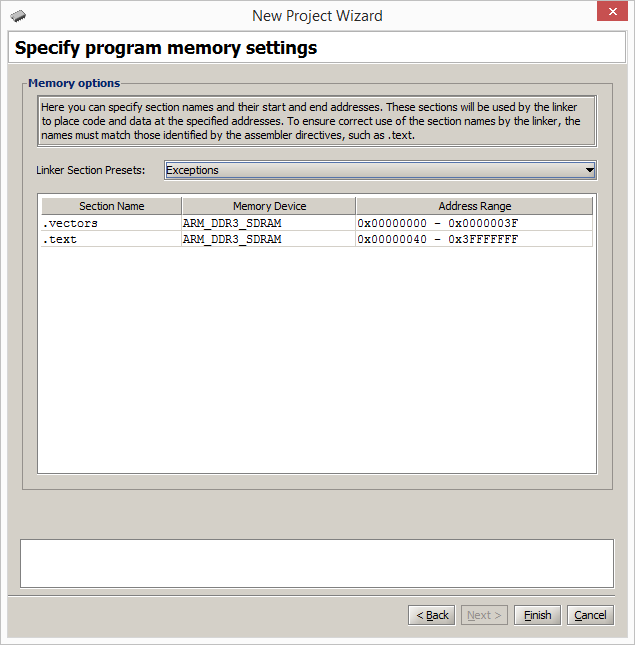
\includegraphics[scale=0.58]{figures/exceptions.png}
	\end{center}
	\vspace{-0.25cm}\caption{Selecting the {\sf Exceptions} linker section.}
\label{fig:exceptions}
\end{figure}

\newpage
\noindent
{\bf Part II}
~\\
~\\
\noindent
Consider the main program shown in Figure~\ref{fig:code2}. The code has to set up 
the ARM processor stack pointers for interrupt and supervisor modes, and then enable interrupts.
The subroutine {\it CONFIG\_GIC} configures the GIC to send interrupts to the ARM processor from
two sources: HPS Timer 0, and the KEY pushbuttons port. The main program calls the
subroutines {\it CONFIG\_HPS\_TIMER} and {\it CONFIG\_KEYS} to set up the two ports. You
are to write each of these subroutines. Set up HPS Timer 0 to generate one interrupt
every 0.25 seconds.

~\\
\noindent
In Figure~\ref{fig:code2} the main program executes an endless loop writing the value of
the global variable {\it COUNT} to the green lights LED.  In the interrupt service routine for 
HPS Timer 0 you are to increment the variable {\it COUNT} by the value of 
the {\it RUN} global variable, 
which should be either 1 or 0.  You are to toggle the value of the {\it RUN} global variable 
in the interrupt service routine for the KEYs, each time a KEY is pressed.
When {\it RUN} = 0, the main program will display a static count on the green lights,
and when {\it RUN} = 1, the count shown on the green lights will increment every 0.25 seconds.

~\\
\noindent
Make a new Monitor Program project for this part, and assemble, download, and test your
code.

~\\
~\\
\noindent
{\bf Part III}
~\\
~\\
\noindent
Modify your program from Part II so that you can vary the speed at which the counter
displayed on the green lights is incremented. All of your changes for this part should be made
in the interrupt service routine for the KEYs. The main program and the rest of
your code should not be changed.

~\\
\noindent
Implement the following behavior. When {\it KEY}$_0$ is pressed, the value of the {\it RUN}
variable should be toggled, as in Part II. Hence, pressing {\it KEY}$_0$ stops/runs
the incrementing of the {\it COUNT} variable. 
When {\it SW}$_0$ is high and {\it KEY}$_1$ is pressed, the rate at which
{\it COUNT} is incremented should be doubled, and when {\it SW}$_0$ is 
low and {\it KEY}$_1$ is pressed the
rate should be halved. You should implement this feature by stopping the HPS Timer within
the KEYs interrupt service routine, modifying the load value used in the
timer, and then restarting the timer.

~\\
~\\
\noindent
{\bf Part IV}
~\\
~\\
\noindent
For this part you are to add a third source of interrupts to your program, using the ARM A9
Private Timer. Set up the timer to provide one interrupt each second. Use this
timer to increment a global variable called {\it TIME}. You should use the {\it TIME} variable as
a real-time clock that is shown on the Monitor Program Terminal window. Use the format 
\blue{MM}:\blue{SS}, where \blue{\it MM} are minutes and \blue{\it SS} are seconds.
You should be able to stop/run the clock by pressing {\it KEY}$_0$.
When the clock reaches \blue{59}:\blue{99}, it should wrap around to \blue{00}:\blue{00}.

\begin{figure}[H]
\begin{center}
\begin{minipage}[t]{16.5 cm}
\lstinputlisting[style=defaultArmStyle]{../design_files/part2.s}
\end{minipage}
\end{center}
\caption{Main program for Part II.}
\label{fig:code2}
\end{figure}

~\\
\noindent
Make a new folder to hold your solution for this part. Modify the main
program from Part~III to call a new subroutine, named {\it CONFIG\_PRIV\_TIMER}, which sets up the
ARM A9 Private Timer to generate the required interrupts. To show the {\it TIME} variable in
the real-time clock format \blue{MM}:\blue{SS}, you can use the approach that was
followed for Part IV of Lab Exercise 4. In Lab Exercise 4 you used polled I/O with
the private timer, whereas now you are using interrupts. The interrupt service routine for
the private timer should display the real-time clock on the Terminal window.

\noindent
Make a new Monitor Program project and test your program. In the screen shown in Figure
\ref{fig:terminal}, make sure to select {\sf JTAG\_UART\_for\_ARM\_0} as the {\it Terminal
device}. Without this setting no character output will appear on the Terminal window when 
your code writes to the JTAG* UART.

~\\
\begin{figure}[htb]
	\begin{center}
	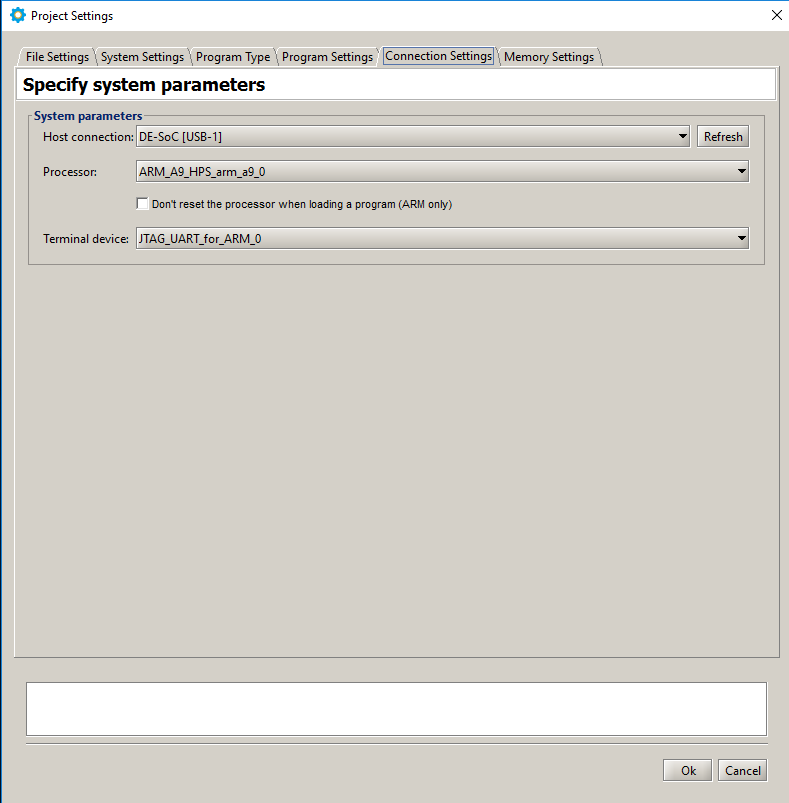
\includegraphics[scale=0.58]{figures/terminal.png}
	\end{center}
	\vspace{-0.25cm}\caption{Specifying the {\it Terminal device}.}
\label{fig:terminal}
\end{figure}

~\\
\noindent
As a final exercise, add to your progam the ability to slow down/speed up the A9 private 
timer, in the same way that you implemented this capability for the HPS Timer in Part III
of this exercise. Observe the behavior of the Terminal window as it displays the real-time 
clock value at various timer rates.  Discuss any anomolous behavior that you observe.


%%%%%%%%%%%%%%%%%%%%%%%%%%%%%%%%%%%%%%%%
%%% FPGAcademy Copyright Information %%%
%%%%%%%%%%%%%%%%%%%%%%%%%%%%%%%%%%%%%%%%

%Always put the copyright on a new page (clear page), with some vertical space from top
\clearpage
\vspace{1in}

\noindent

Copyright {\copyright} FPGAcademy.org. All rights reserved. FPGAcademy and the 
FPGAcademy logo are trademarks of FPGAcademy.org.  This document is provided 
"as is", without warranty of any kind, express or implied, including but not 
limited to the warranties of merchantability, fitness for a particular purpose 
and noninfringement. In no event shall the authors or copyright holders be 
liable for any claim, damages or other liability, whether in an action of 
contract, tort or otherwise, arising from, out of or in connection with the 
document or the use or other dealings in the document.
~\\
~\\
**Other names and brands may be claimed as the property of others.


\end{document}
